\documentclass{ximera}

%% You can put user macros here
%% However, you cannot make new environments

\listfiles

\graphicspath{{./}{firstExample/}{secondExample/}}

\usepackage{tikz}
\usepackage{tkz-euclide}
\usepackage{tikz-3dplot}
\usepackage{tikz-cd}
\usetikzlibrary{shapes.geometric}
\usetikzlibrary{arrows}
\usetikzlibrary{decorations.pathmorphing,patterns}
\usetkzobj{all}
\pgfplotsset{compat=1.13} % prevents compile error.

\renewcommand{\vec}[1]{\mathbf{#1}}
\newcommand{\RR}{\mathbb{R}}
\newcommand{\dfn}{\textit}
\newcommand{\dotp}{\cdot}
\newcommand{\id}{\text{id}}
\newcommand\norm[1]{\left\lVert#1\right\rVert}
 
\newtheorem{general}{Generalization}
\newtheorem{initprob}{Exploration Problem}

\tikzstyle geometryDiagrams=[ultra thick,color=blue!50!black]

\usepackage{mathtools}

\title{Introduction to the Laplace Transform}%\label{Module 7-ADEF}

\begin{document}

\begin{abstract}
We begin our study of Laplace transforms with the definition, and we derive the Laplace Transform of some basic functions.
\end{abstract}

\maketitle

\section*{Introduction to the Laplace Transform}

\subsection*{Definition of the Laplace Transform}

 
To define the Laplace transform, we first recall the definition of an
improper integral. If $g$ is integrable over the
interval $[a,T]$ for every $T>a$, then the \textit{improper
integral of
$g$ over} $[a,\infty)$ is defined as
\begin{equation} \label{eq:8.1.1}
\int^\infty_a g(t)\,dt=\lim_{T\rightarrow\infty}\int^T_a g(t)\,dt.
\end{equation}
We say that the improper integral \textit{converges} if the limit in
\eqref{eq:8.1.1} exists;   otherwise, we say that the improper integral
\textit{diverges} or \textit{does not exist}. Here's the definition of
the Laplace transform of a function $f$.

\begin{definition}\label{thmtype:8.1.1}
Let $f$ be defined for $t\geq 0$ and let $s$ be a real number. Then the
\href{http://www-history.mcs.st-and.ac.uk/Mathematicians/Laplace.html}{Laplace transform} of $f$ is the function $F$ defined by
\begin{equation}\label{eq:8.1.2} F(s)=\int_0^\infty e^{-st} f(t)\,dt,
\end{equation} for those values of $s$ for which the improper integral
converges.
\end{definition}

It is important to keep in mind that the variable of integration in
\eqref{eq:8.1.2} is $t$, while $s$ is a parameter independent of $t$. We
use $t$ as the independent variable for $f$ because in applications
the Laplace transform is usually applied to functions of time.

The Laplace transform can be viewed as an operator ${\cal L}$ that
transforms the function $f=f(t)$  into the function $F=F(s)$. Thus,
\eqref{eq:8.1.2} can be expressed as
$$
F={\cal L}(f).
$$
The functions $f$ and $F$ form a \textit{transform pair}, which we'll
sometimes denote by
$$
f(t)\leftrightarrow F(s).
$$
It can be shown that if $F(s)$ is defined for $s=s_0$ then it's defined
for all $s>s_0$. %(Exercise~\ref{exer:8.1.14}\part{b}).

\subsection*{Computation of Some Simple Laplace Transforms}

\begin{example}\label{example:8.1.1} 
 Find the Laplace transform of  $f(t)=1$.


\begin{explanation}
 From  \eqref{eq:8.1.2} with $f(t)=1$,
$$
F(s)=\int_0^\infty e^{-st}\,dt=\lim_{T\rightarrow\infty}\int_0^T e^{-st}\,
dt.
$$
If $s\neq 0$ then
\begin{equation}\label{eq:8.1.3}
\int_0^T e^{-st}dt=-\frac{1}{s}e^{-st}\Big|_0^T=\frac{1-e^{-sT}}{s}.
\end{equation}
Therefore
\begin{equation}\label{eq:8.1.4}
\lim_{T\rightarrow\infty}\int_0^T e^{-st}dt=\left\{\begin{array}{rr}
\frac{1}{s}, &   s>0,\\
\infty, &  s<0.
\end{array}\right.
\end{equation}
If $s=0$  the integrand reduces to the constant $1$, and
$$
\lim_{T\rightarrow\infty}\int_0^T 1\,dt=\lim_{T\rightarrow\infty}\int_0^T 1\,dt=
\lim_{T\rightarrow\infty}T=\infty.
$$
Therefore $F(0)$ is undefined, and
$$
F(s)=\int_0^\infty e^{-st}dt=\frac{1}{s},\quad s>0.
$$
This result can be written in operator notation as
$$
{\cal L}(1)=\frac{1}{s},\quad s>0,
$$
or as the transform pair
$$
1\leftrightarrow\frac{1}{s},\quad s>0.
$$
\end{explanation}
\end{example}
\begin{remark}
It is convenient to combine the steps of integrating from $0$ to $T$
and letting $T\rightarrow\infty$. Therefore, instead of writing \eqref{eq:8.1.3}
and \eqref{eq:8.1.4} as separate steps we write
$$
\int_0^\infty e^{-st}dt=-\frac{1}{s} e^{-st}\Big|_0^\infty=
\left\{\begin{array}{rr}\frac{1}{s}, & s>0,\\\infty,&s<
0.\end{array}\right.
$$
We'll follow this practice throughout this chapter.
\end{remark}

\begin{example}\label{example:8.1.2}
 Find the Laplace transform of $f(t)=t$.
\begin{explanation}
  From  \eqref{eq:8.1.2} with $f(t)=t$,
\begin{equation}\label{eq:8.1.5}
F(s)=\int_0^\infty e^{-st}t\,dt.
\end{equation}
If $s\neq 0$,  integrating by parts yields
\begin{eqnarray*}
\int_0^\infty e^{-st}t\,dt&=&-\frac{te^{-st}}{s}\bigg|_0^\infty
+\frac{1}{s}\int_0^\infty e^{-st}\,dt
=-\left[\frac{t}{s}+\frac{1}{s^2}\right]e^{-st}\bigg|_0^\infty
\\&=&\left\{\begin{array}{rr}\frac{1}{s^2},\quad s>0,\\
\infty,\,s<0.\end{array}\right.
\end{eqnarray*}
If $s=0$, the integral in  \eqref{eq:8.1.5} becomes
$$
\int_0^\infty t\,dt=\frac{t^2}{2}\bigg|_0^\infty=\infty.
$$
Therefore $F(0)$ is undefined and
$$
F(s)=\frac{1}{s^2},\quad s>0.
$$
This result can also be written as
$$
{\cal L}(t)=\frac{1}{s^2},\quad s>0,
$$
or as the transform pair
$$
t\leftrightarrow\frac{1}{s^2},\quad s>0.
$$
\end{explanation}
\end{example}

\begin{example}\label{example:8.1.3}
 Find the Laplace transform of $f(t)=e^{at}$, where $a$ is a constant.
\begin{explanation}
From  \eqref{eq:8.1.2} with $f(t)=e^{at}$,
$$
F(s)=\int_0^\infty e^{-st}e^{at}\,dt.
$$
Combining the exponentials yields
$$
F(s)=\int_0^\infty e^{-(s-a)t}\,dt.
$$
However, we know from Example~\ref{example:8.1.1}  that
$$
\int_0^\infty e^{-st}\,dt=\frac{1}{s},\quad s>0.
$$
Replacing $s$ by $s-a$ here shows that
$$
F(s)=\frac{1}{s-a},\quad s>a.
$$
This can also be written as
$$
{\cal L}(e^{at})=\frac{1}{s-a},\quad s>a, \quad\text{or}\quad
 e^{at}\leftrightarrow\frac{1}{s-a},\quad s>a.
$$
\end{explanation}
\end{example}



\begin{example}\label{example:8.1.4} 
Find the Laplace transforms of $f(t)=\sin\omega t$ and
$g(t)=\cos\omega t$, where $\omega$ is a constant.

\begin{explanation}  
Define
\begin{equation}\label{eq:8.1.6}
F(s)=\int_0^\infty e^{-st}\sin\omega t\,dt
\end{equation}
and
\begin{equation}\label{eq:8.1.7}
G(s)=\int_0^\infty e^{-st}\cos\omega t\,dt.
\end{equation}
If $s>0$, integrating  \eqref{eq:8.1.6} by parts yields
$$
F(s)=-\frac{e^{-st}}{s}\sin\omega t\Big|_0^\infty+\frac{\omega}{s}
\int_0^\infty e^{-st}\cos\omega t\,dt,
$$
so
\begin{equation}\label{eq:8.1.8}
F(s)=\frac{\omega}{s}G(s).
\end{equation}
If $s>0$, integrating  \eqref{eq:8.1.7} by parts yields
$$
G(s)=-\frac{e^{-st}\cos\omega t}{s}\Big|_0^\infty - \frac{\omega}{s}
\int_0^\infty e^{-st}\sin\omega t\,dt,
$$
so
$$
G(s)=\frac{1}{s} - \frac{\omega}{s} F(s).
$$
Now substitute from  \eqref{eq:8.1.8} into this to obtain
$$
G(s)=\frac{1}{s} - \frac{\omega^2}{s^2} G(s).
$$
Solving this for $G(s)$ yields
$$
G(s)=\frac{s}{s^2+\omega^2},\quad s>0.
$$
This and  \eqref{eq:8.1.8} imply that
$$
F(s)=\frac{\omega}{s^2+\omega^2},\quad s>0.
$$
\end{explanation}
\end{example}
\subsection*{Tables of Laplace transforms}

Extensive tables of Laplace transforms have been compiled and are
commonly used in applications. The brief table of Laplace transforms
in \href{https://ximera.osu.edu/ode/main/laplaceTable/laplaceTable}{Trench 8.8} 
will be adequate for our purposes.

\begin{example}\label{example:8.1.5}  Use the
table of Laplace transforms to find  ${\cal L}(t^3e^{4t})$.

\begin{explanation}
The table includes the transform pair
$$
t^ne^{at}\leftrightarrow \frac{n!}{(s-a)^{n+1}}.
$$
Setting $n=3$ and $a=4$ here yields
$$
{\cal L}(t^3e^{4t})=\frac{3!}{(s-4)^4}=\frac{6}{(s-4)^4}.
$$
\end{explanation}
\end{example}

We'll sometimes write Laplace transforms of specific functions
without explicitly stating how they are obtained. In such cases you
should refer to the table of Laplace transforms.

\subsection*{Linearity of the Laplace Transform}

The next theorem presents an important property of the Laplace
transform.

\begin{theorem}[Linearity Property]\label{thmtype:8.1.2}
 Suppose ${\cal L}(f_i)$ is defined for
 $s>s_i,$ $1\leq i\leq n)$.
Let $s_0$ be the largest of the numbers $s_1, s_{2}, \dots,s_n,$ and
let
$c_1, c_2,\dots, c_n$ be  constants. Then
$$
{\cal L}(c_1f_1+c_2f_2+\cdots+c_nf_n)=c_1{\cal L}(f_1)+c_2{\cal L}(f_2)
+\cdots+c_n{\cal L}(f_n)\mbox{ for } s>s_0.
$$
\end{theorem}

\begin{proof}
We give the proof for the case where $n=2$. If $s>s_0$ then
\begin{eqnarray*}
{\cal L}(c_1f_1+c_2f_2)&=&
\int_0^\infty
e^{-st}\left(c_1f_1(t)+c_2f_2(t))\right)\,dt\\
&=&c_1\int_0^\infty e^{-st}f_1(t)\,dt+c_2\int_0^\infty e^{-st}f_2(t)\,dt\\
&=&c_1{\cal L}(f_1)+c_2{\cal L}(f_2).
\end{eqnarray*}
\end{proof}

\begin{example}\label{example:8.1.6}
Use  Theorem~\ref{thmtype:8.1.2} and the known Laplace transform
$$
{\cal L}(e^{at})=\frac{1}{s-a}
$$
 to find ${\cal L}(\cosh bt)\,(b\neq 0)$.


\begin{explanation}  By definition,
$$
\cosh bt=\frac{e^{bt}+e^{-bt}}{2}.
$$
Therefore
\begin{equation}\label{eq:8.1.9}
\begin{array}{ccl}
{\cal L}(\cosh bt)&=& {\cal L}\left(\frac{1}{2} e^{bt}+\frac{1}{2}e^{-bt}\right)\\%[2\jot]
&=&\frac{1}{2} {\cal L}(e^{bt}) +\frac{1}{2} {\cal L}(e^{-bt})
\qquad
\mbox{(linearity property)}\\%[2\jot]
&=&\frac{1}{2}\,\frac{1}{s-b} +\frac{1}{2}\,\frac{1}{s+b},
\end{array}
\end{equation}
where the first transform on the right is defined for $s>b$ and the
second
for $s>-b$; hence, both are defined for $s>|b|$.  Simplifying the
last expression in \eqref{eq:8.1.9} yields
$$
{\cal L}(\cosh bt)=\frac{s}{s^2-b^2},\quad s>|b|.
$$
\end{explanation}
\end{example}

\subsection*{The First Shifting Theorem}

The next theorem enables us to start with known transform pairs and derive
others. 
%(For other results of this kind, see Exercises~\ref{exer:8.1.6}  and
%\ref{exer:8.1.13}.)

\begin{theorem}[First Shifting
Theorem]\label{thmtype:8.1.3}
 If
\begin{equation}\label{eq:8.1.10}
F(s)=\int_0^\infty e^{-st} f(t)\,dt
\end{equation}
is the Laplace transform of $f(t)$ for $s>s_0$, then $F(s-a)$ is the
Laplace transform of $e^{at}f(t)$ for $s >s_0+a$.
\end{theorem}

\begin{proof}
Replacing $s$ by $s-a$ in  \eqref{eq:8.1.10} yields
\begin{equation}\label{eq:8.1.11}
F(s-a)=\int_0^\infty e^{-(s-a)t}f(t)\,dt
\end{equation}
if $s-a>s_0$; that is, if $s>s_0+a$.  However,  \eqref{eq:8.1.11} can
be rewritten as
$$
F(s-a)=\int_0^\infty e^{-st}\left(e^{at}f(t)\right)\,dt,
$$
which implies the conclusion.
\end{proof}

\begin{example}\label{example:8.1.7}
  Use Theorem~\ref{thmtype:8.1.3} and the known Laplace
transforms of $1$, $t$, $\cos\omega t$, and $\sin\omega t$ to find
$$
{\cal L}(e^{at}),\quad {\cal L}(te^{at}),\quad {\cal L}(e^{\lambda t}\sin
\omega t),\mbox{and } {\cal L}(e^{\lambda t}\cos\omega t).
$$
\begin{explanation}
In the following table the known
transform pairs  are listed on the left and  the required  transform pairs
listed on the right are obtained  by applying
Theorem~\ref{thmtype:8.1.3}.

\begin{center}
\begin{tabular}{|c|c|}\hline
$f(t)\leftrightarrow F(s)$ & $e^{at}f(t)\leftrightarrow F(s-a)$ \\\hline
&\\ $1\leftrightarrow\frac{1}{s},\quad s>0$ &
 $e^{at}\leftrightarrow\frac{1}{(s-a)},\quad s>a$\\
  $t\leftrightarrow\frac{{1}{s^2}},\quad s>0$ &
$te^{at}\leftrightarrow\frac{{1}{(s-a)^2}},\quad s>a$\\
$\sin\omega t\leftrightarrow\frac{{\omega}{s^2+\omega^2}},\quad s>0$&
$e^{\lambda t}\sin\omega t\leftrightarrow\frac{{\omega}{(s-\lambda)^2+\omega^2}},\,s>\lambda$\\
$\cos\omega t\leftrightarrow\frac{{s}{s^2+\omega^2}},\quad s>0$ &
$e^{\lambda t}\sin\omega t\leftrightarrow\frac{{s-\lambda}{(s-\lambda)^2+\omega^2}},\,s>\lambda$\\\hline
\end{tabular}
\end{center}
\end{explanation}
\end{example}



\subsection*{Existence of Laplace Transforms}

Not every function has a Laplace transform.  For example, it can be shown
%(Exercise~\ref{exer:8.1.3}) 
that
$$
\int_0^\infty e^{-st}e^{t^2} dt=\infty
$$
for every real number $s$. Hence, the function $f(t)=e^{t^2}$ does not
have a Laplace transform.

Our next objective is to establish conditions that ensure the
existence of the Laplace transform of a function. We first review some
relevant definitions from calculus.

Recall that a limit
$$
\lim_{t\rightarrow t_0} f(t)
$$
exists if and only if the one-sided limits
$$
\lim_{t\rightarrow t_0-}f(t)\quad\mbox{and}\quad\lim_{t\rightarrow t_0+}f(t)
$$
  both exist and are equal;   in this case,
$$
\lim_{t\rightarrow t_0}f(t)=\lim_{t\rightarrow t_0-}f(t)=\lim_{t\rightarrow t_0+}f(t) .
$$
Recall also that $f$ is continuous at a point $t_0$ in an open interval
$(a,b)$ if and only if
$$
\lim_{t\rightarrow t_0}f(t)=f(t_0),
$$
which is  equivalent to
\begin{equation}\label{eq:8.1.12}
\lim_{t\rightarrow t_0+}f(t)=\lim_{t\rightarrow t_0-}f(t)=f(t_0).
\end{equation}
For simplicity, we  define
$$
f(t_0+)=\lim_{t\rightarrow t_0+}f(t)\quad\mbox{and}\quad f(t_0-)=\lim_{t\rightarrow
t_0-}f(t),
$$
so  \eqref{eq:8.1.12} can be expressed as
$$
f(t_0+)=f(t_0-)=f(t_0).
$$
If $f(t_0+)$ and $f(t_0-)$ have finite but distinct values,  we say
that $f$ has a \textit{jump discontinuity}  at $t_0$,
 and
$$
f(t_0+)-f(t_0-)
$$
is called the \textit{jump} in $f$ at $t_0$ the figure below.

\begin{image}
 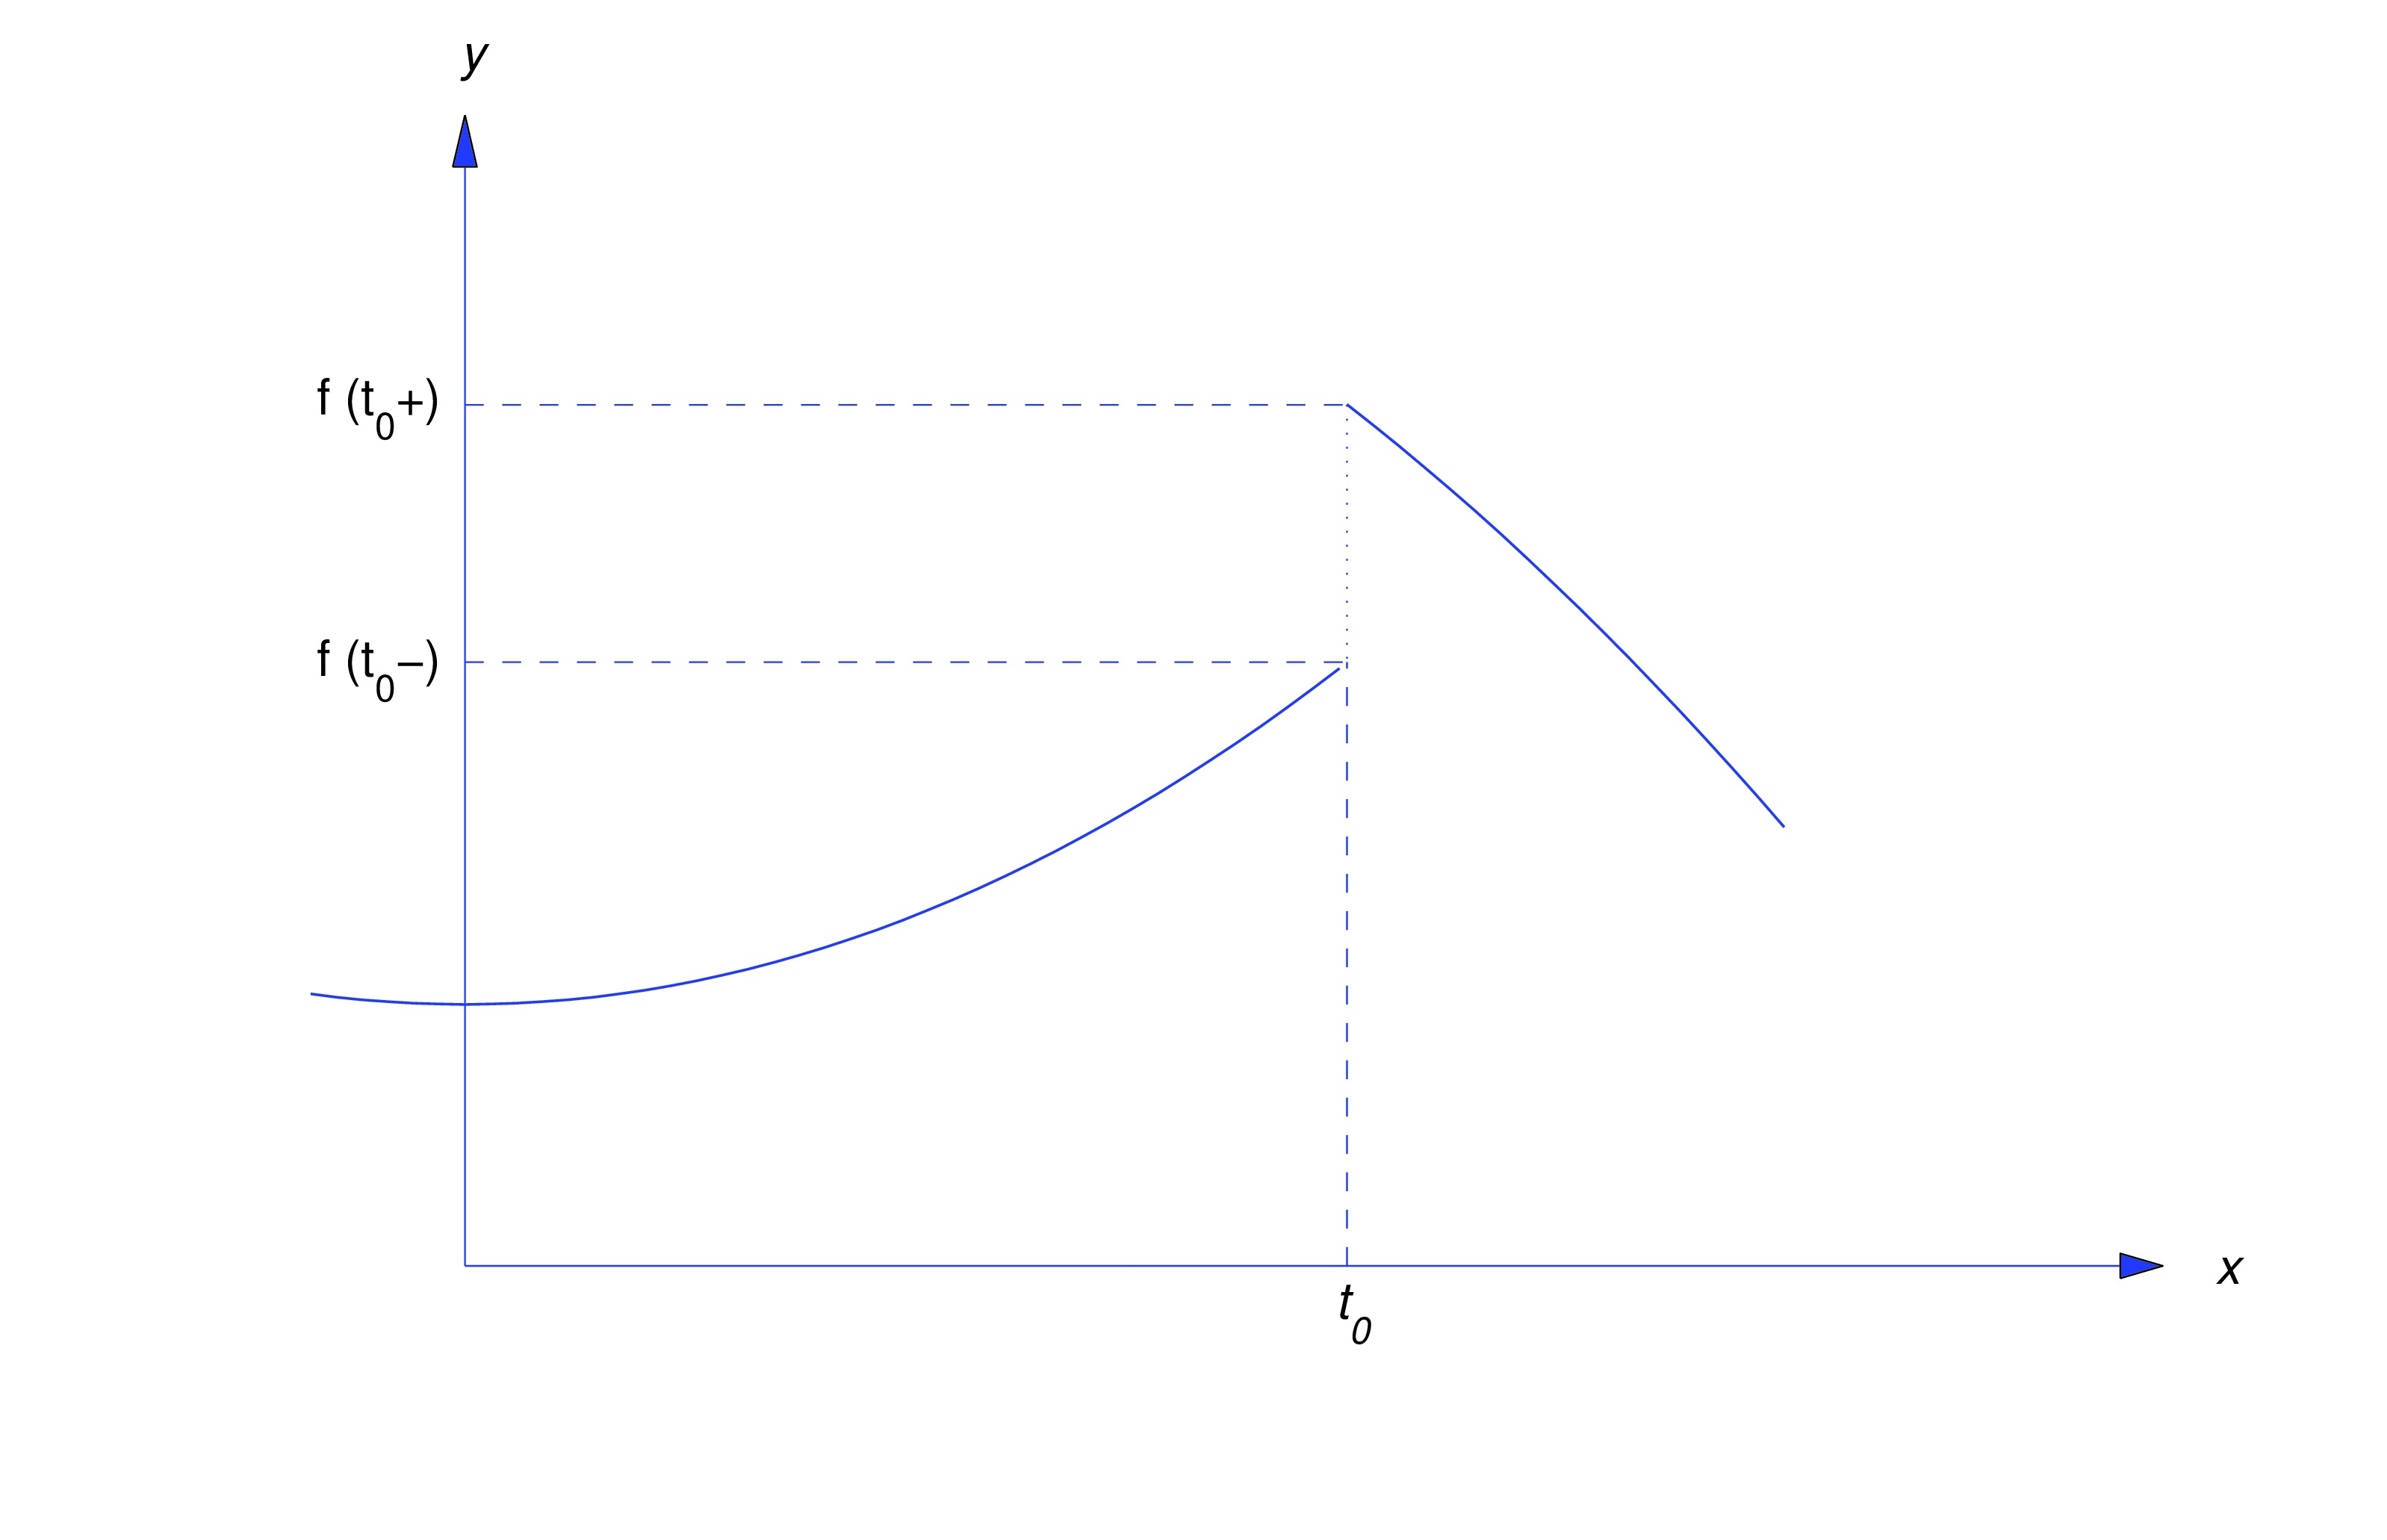
\includegraphics[height=1.5in]{fig080101.jpg}
\end{image}

% \
% \begin{figure}[tbp]
%   \centering\color{blue}
%   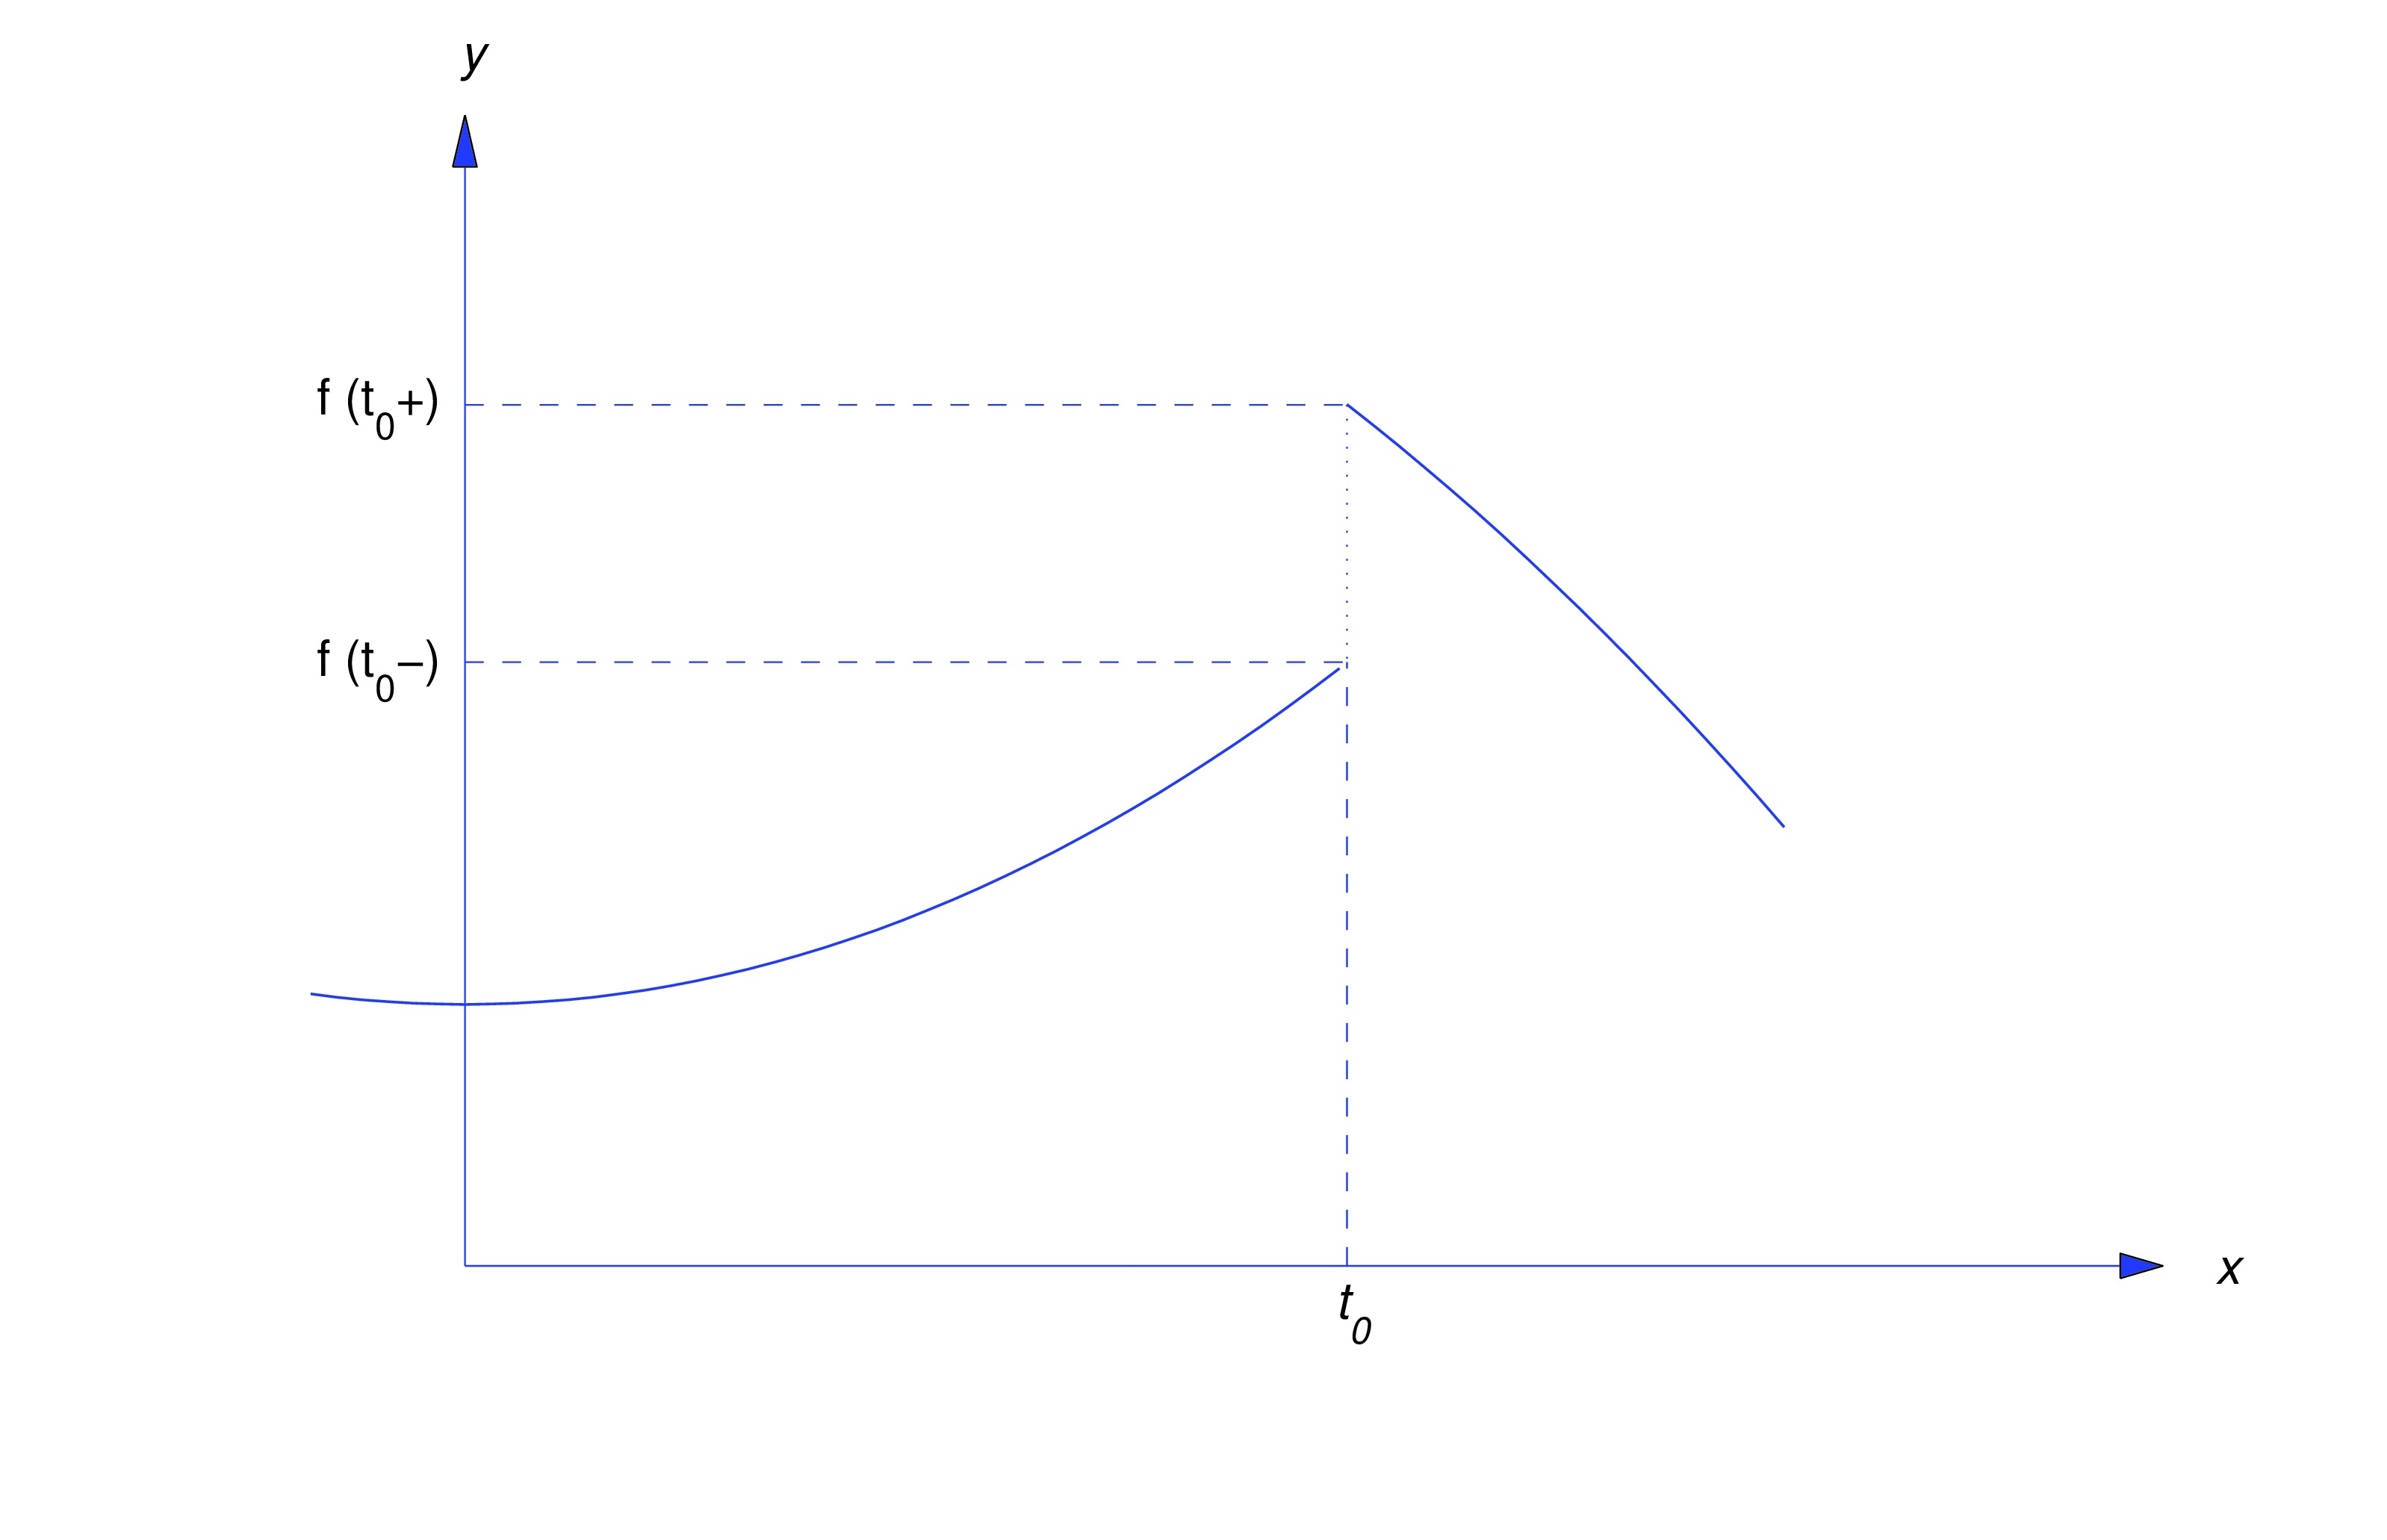
\includegraphics[bb=-78 148 689 643,width=5.67in,height=3.66in,keepaspectratio]{fig080101}
% \caption{ A jump discontinuity}
%   \label{figure:8.1.1}
% \end{figure}

If $f(t_0+)$ and $f(t_0-)$ are finite and equal, but either $f$ isn't
defined at $t_0$ or it's defined but
$$
f(t_0)\neq f(t_0+)=f(t_0-),
$$
 we say that $f$ has a \textit{removable discontinuity} at $t_0$
(see the figure below).%(Figure~\ref{figure:8.1.2}).
This terminology is appropriate since a function $f$  with a removable
discontinuity at $t_0$  can be made continuous at $t_0$ by defining (or
redefining)
$$
f(t_0)=f(t_0+)=f(t_0-).
$$

\begin{image}
 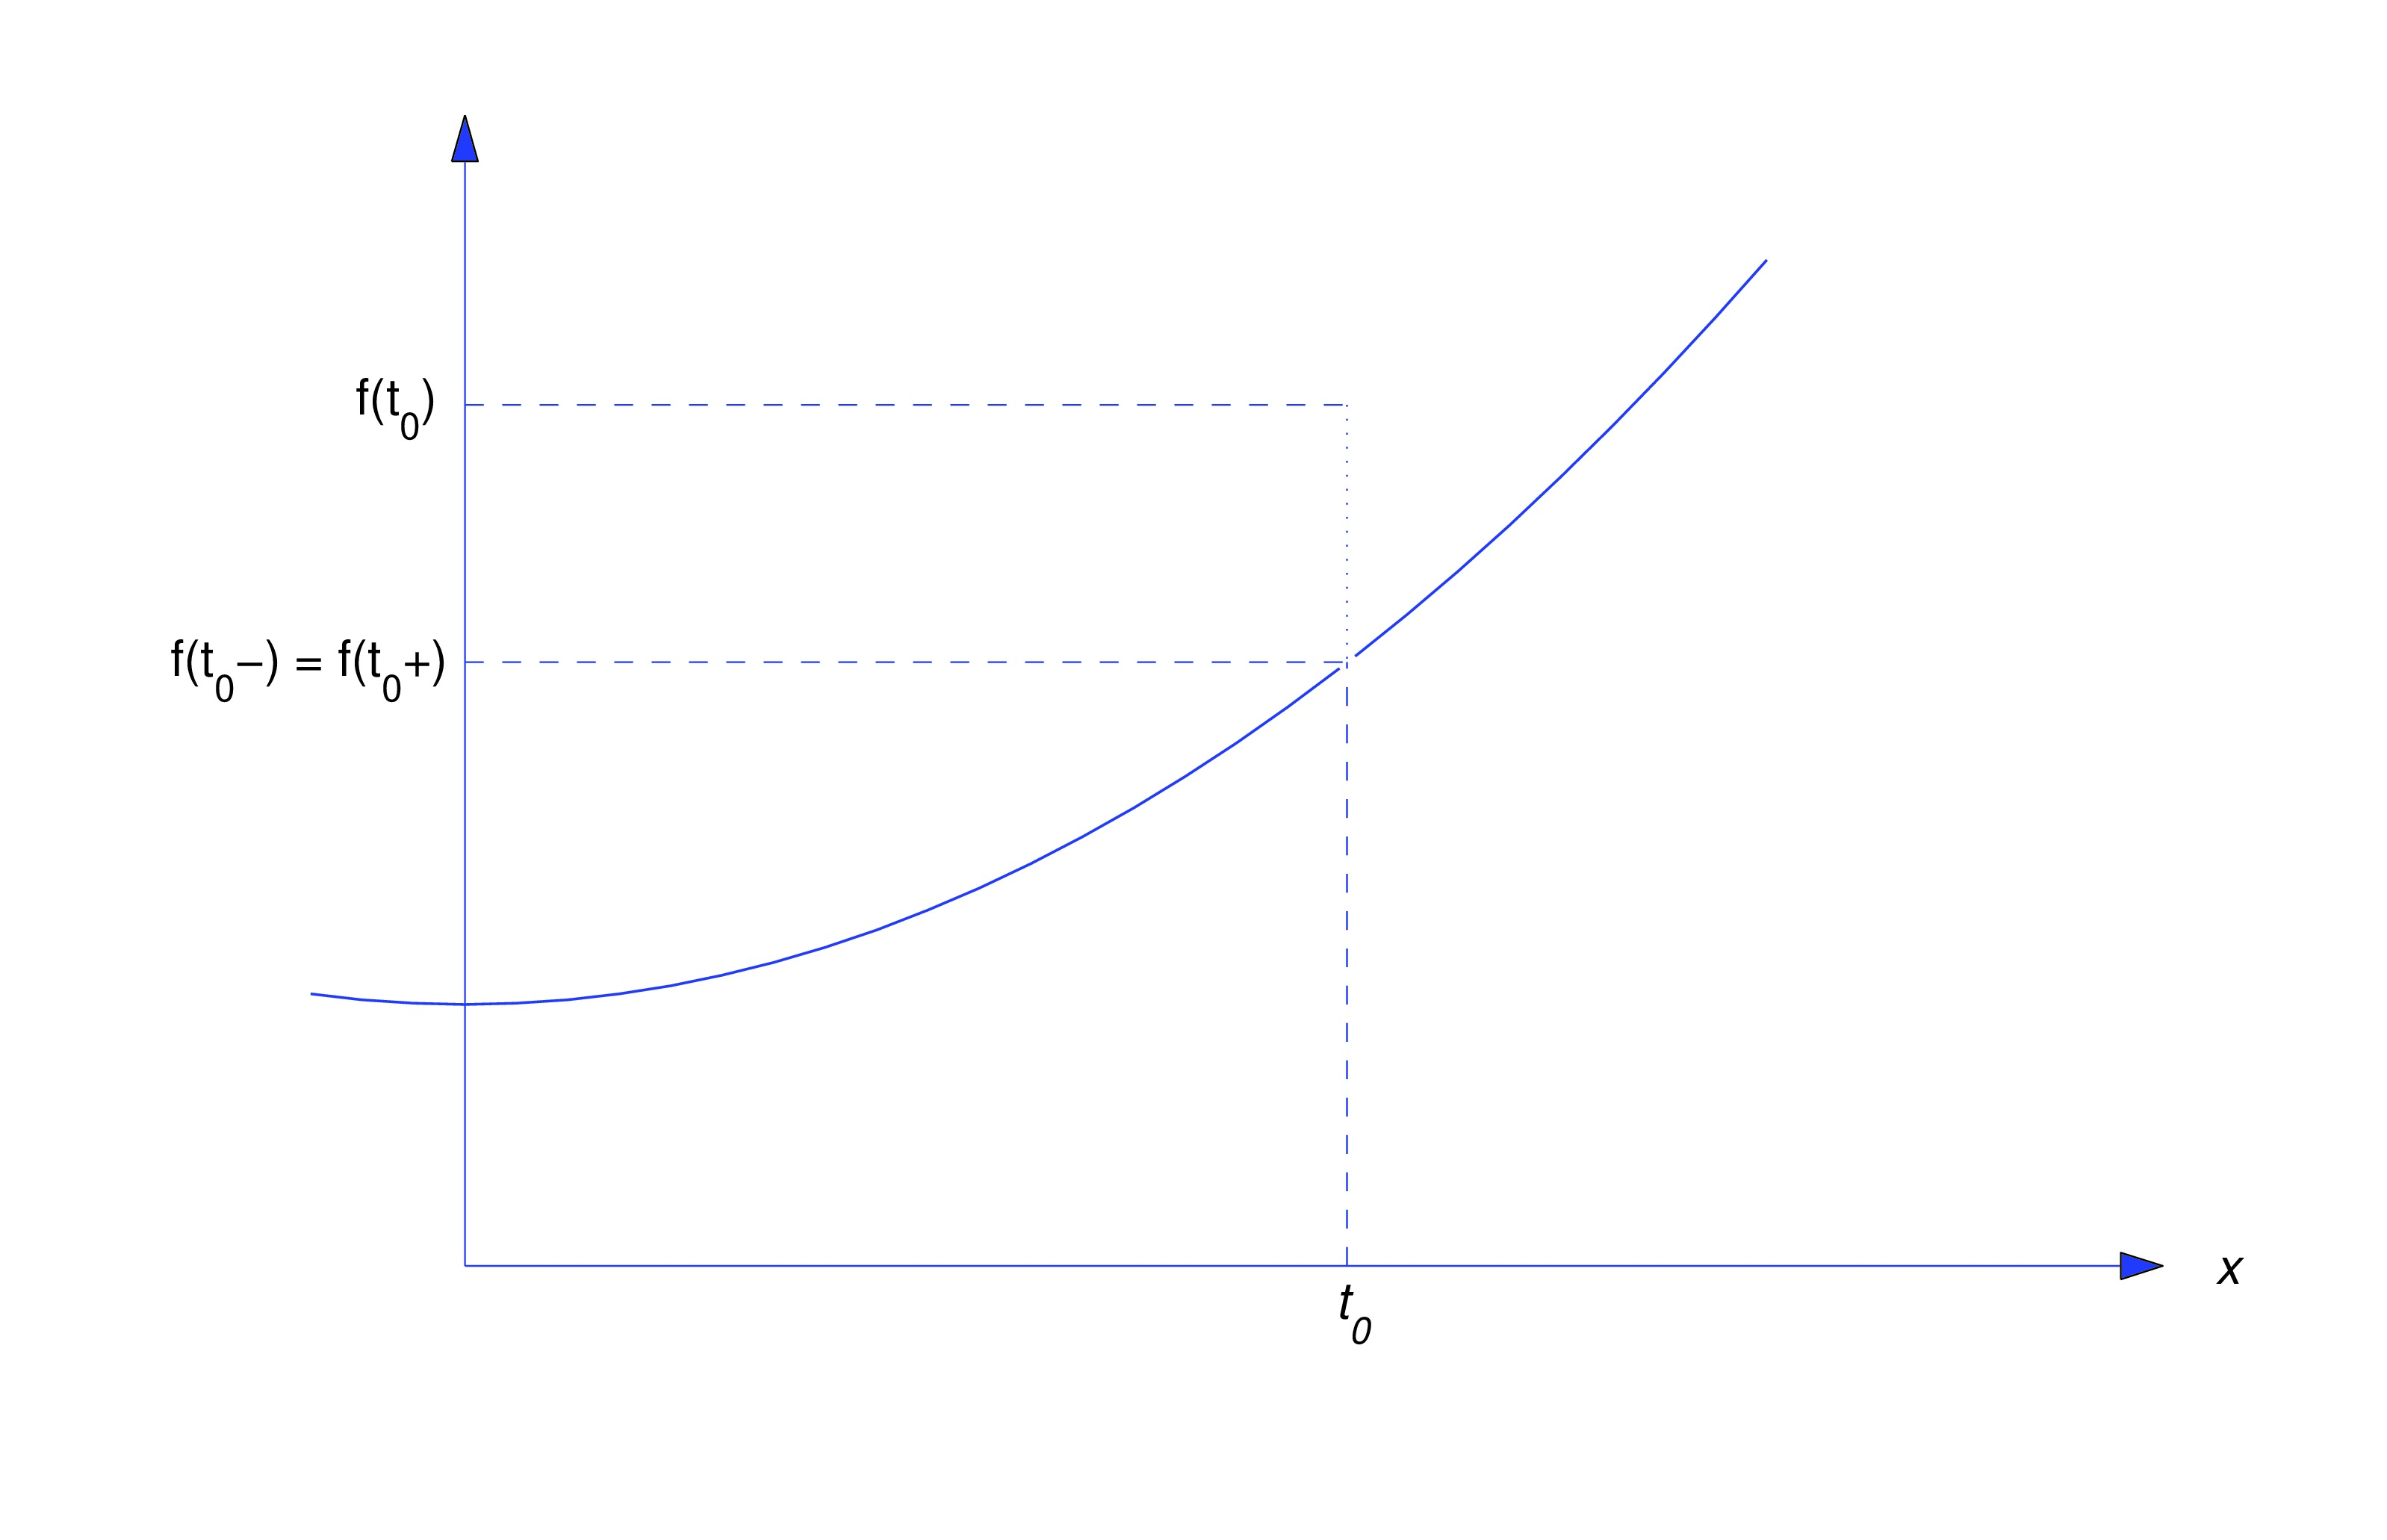
\includegraphics[height=1.5in]{fig080102.jpg}
 \end{image}

% \begin{figure}[htbp]
% \color{blue}
%   \begin{minipage}[b]{0.5\linewidth}
%     \centering
%   \scalebox{.65}{
%   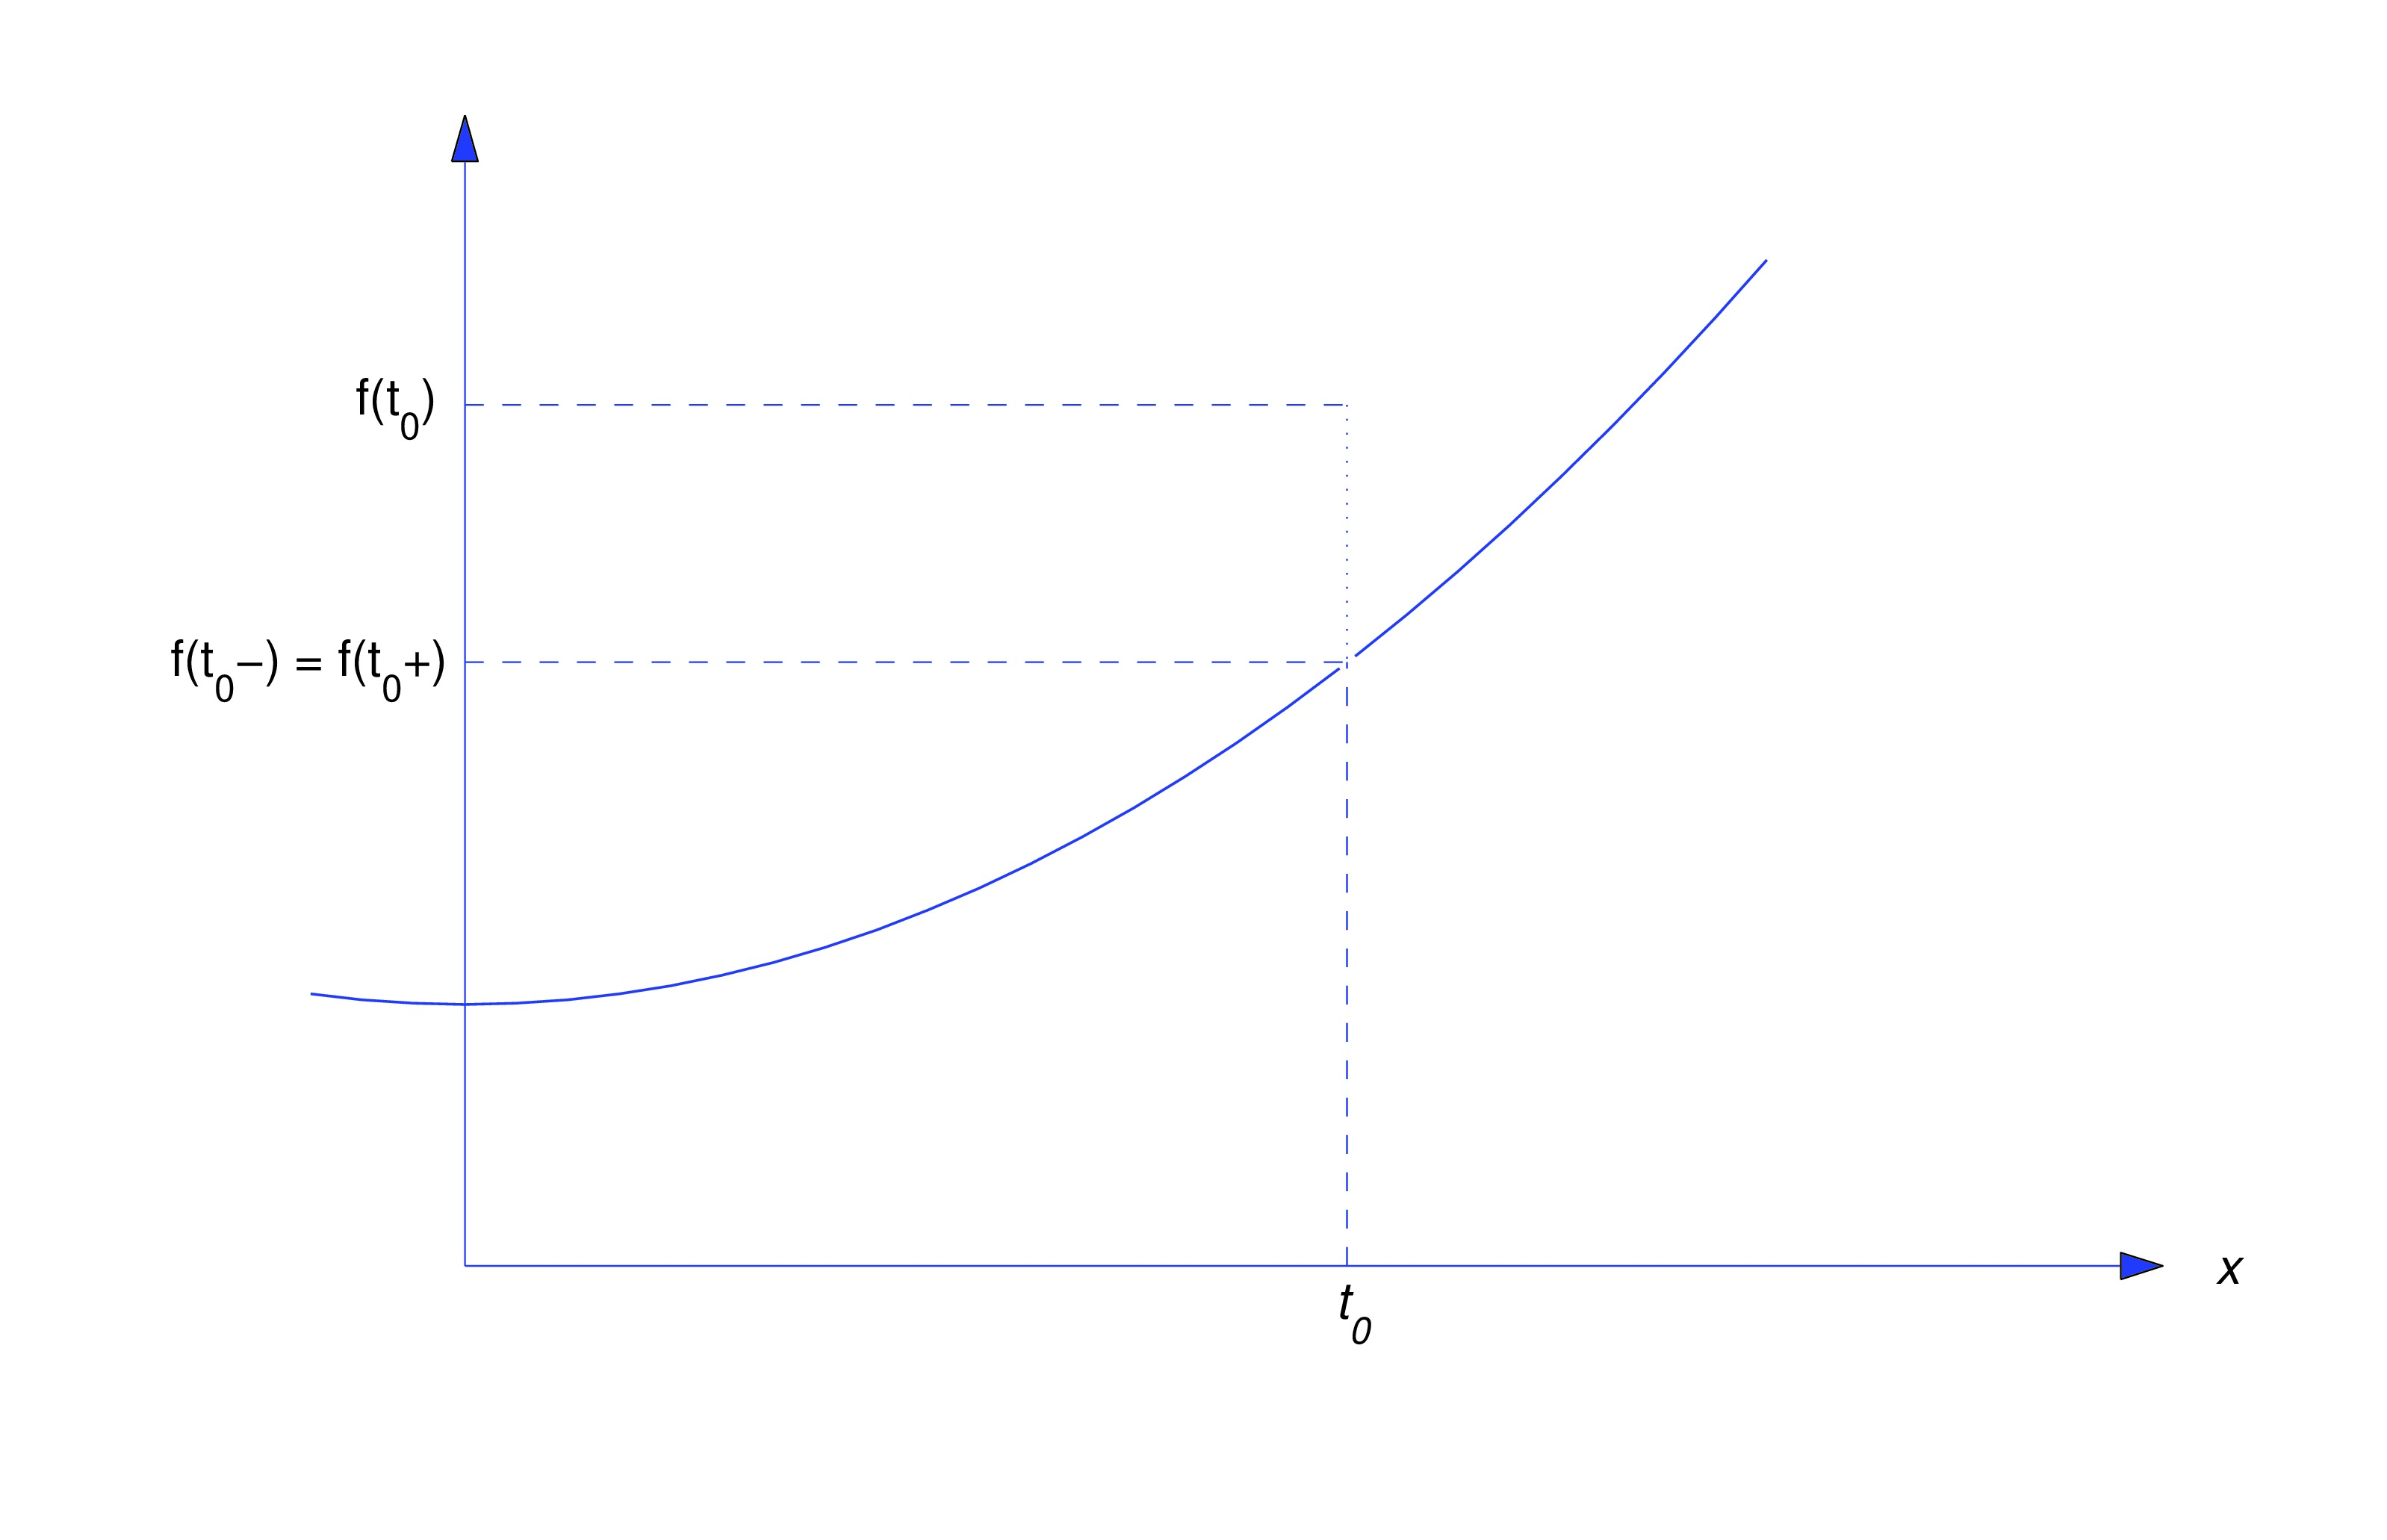
\includegraphics[bb=-78 148 689 643,width=5.67in,height=3.66in,keepaspectratio]{fig080102}}
%   \caption{}
%   \label{figure:8.1.2}
% \end{minipage}
%   \begin{minipage}[b]{0.5\linewidth}
%     \centering
%   \scalebox{.65}{
%   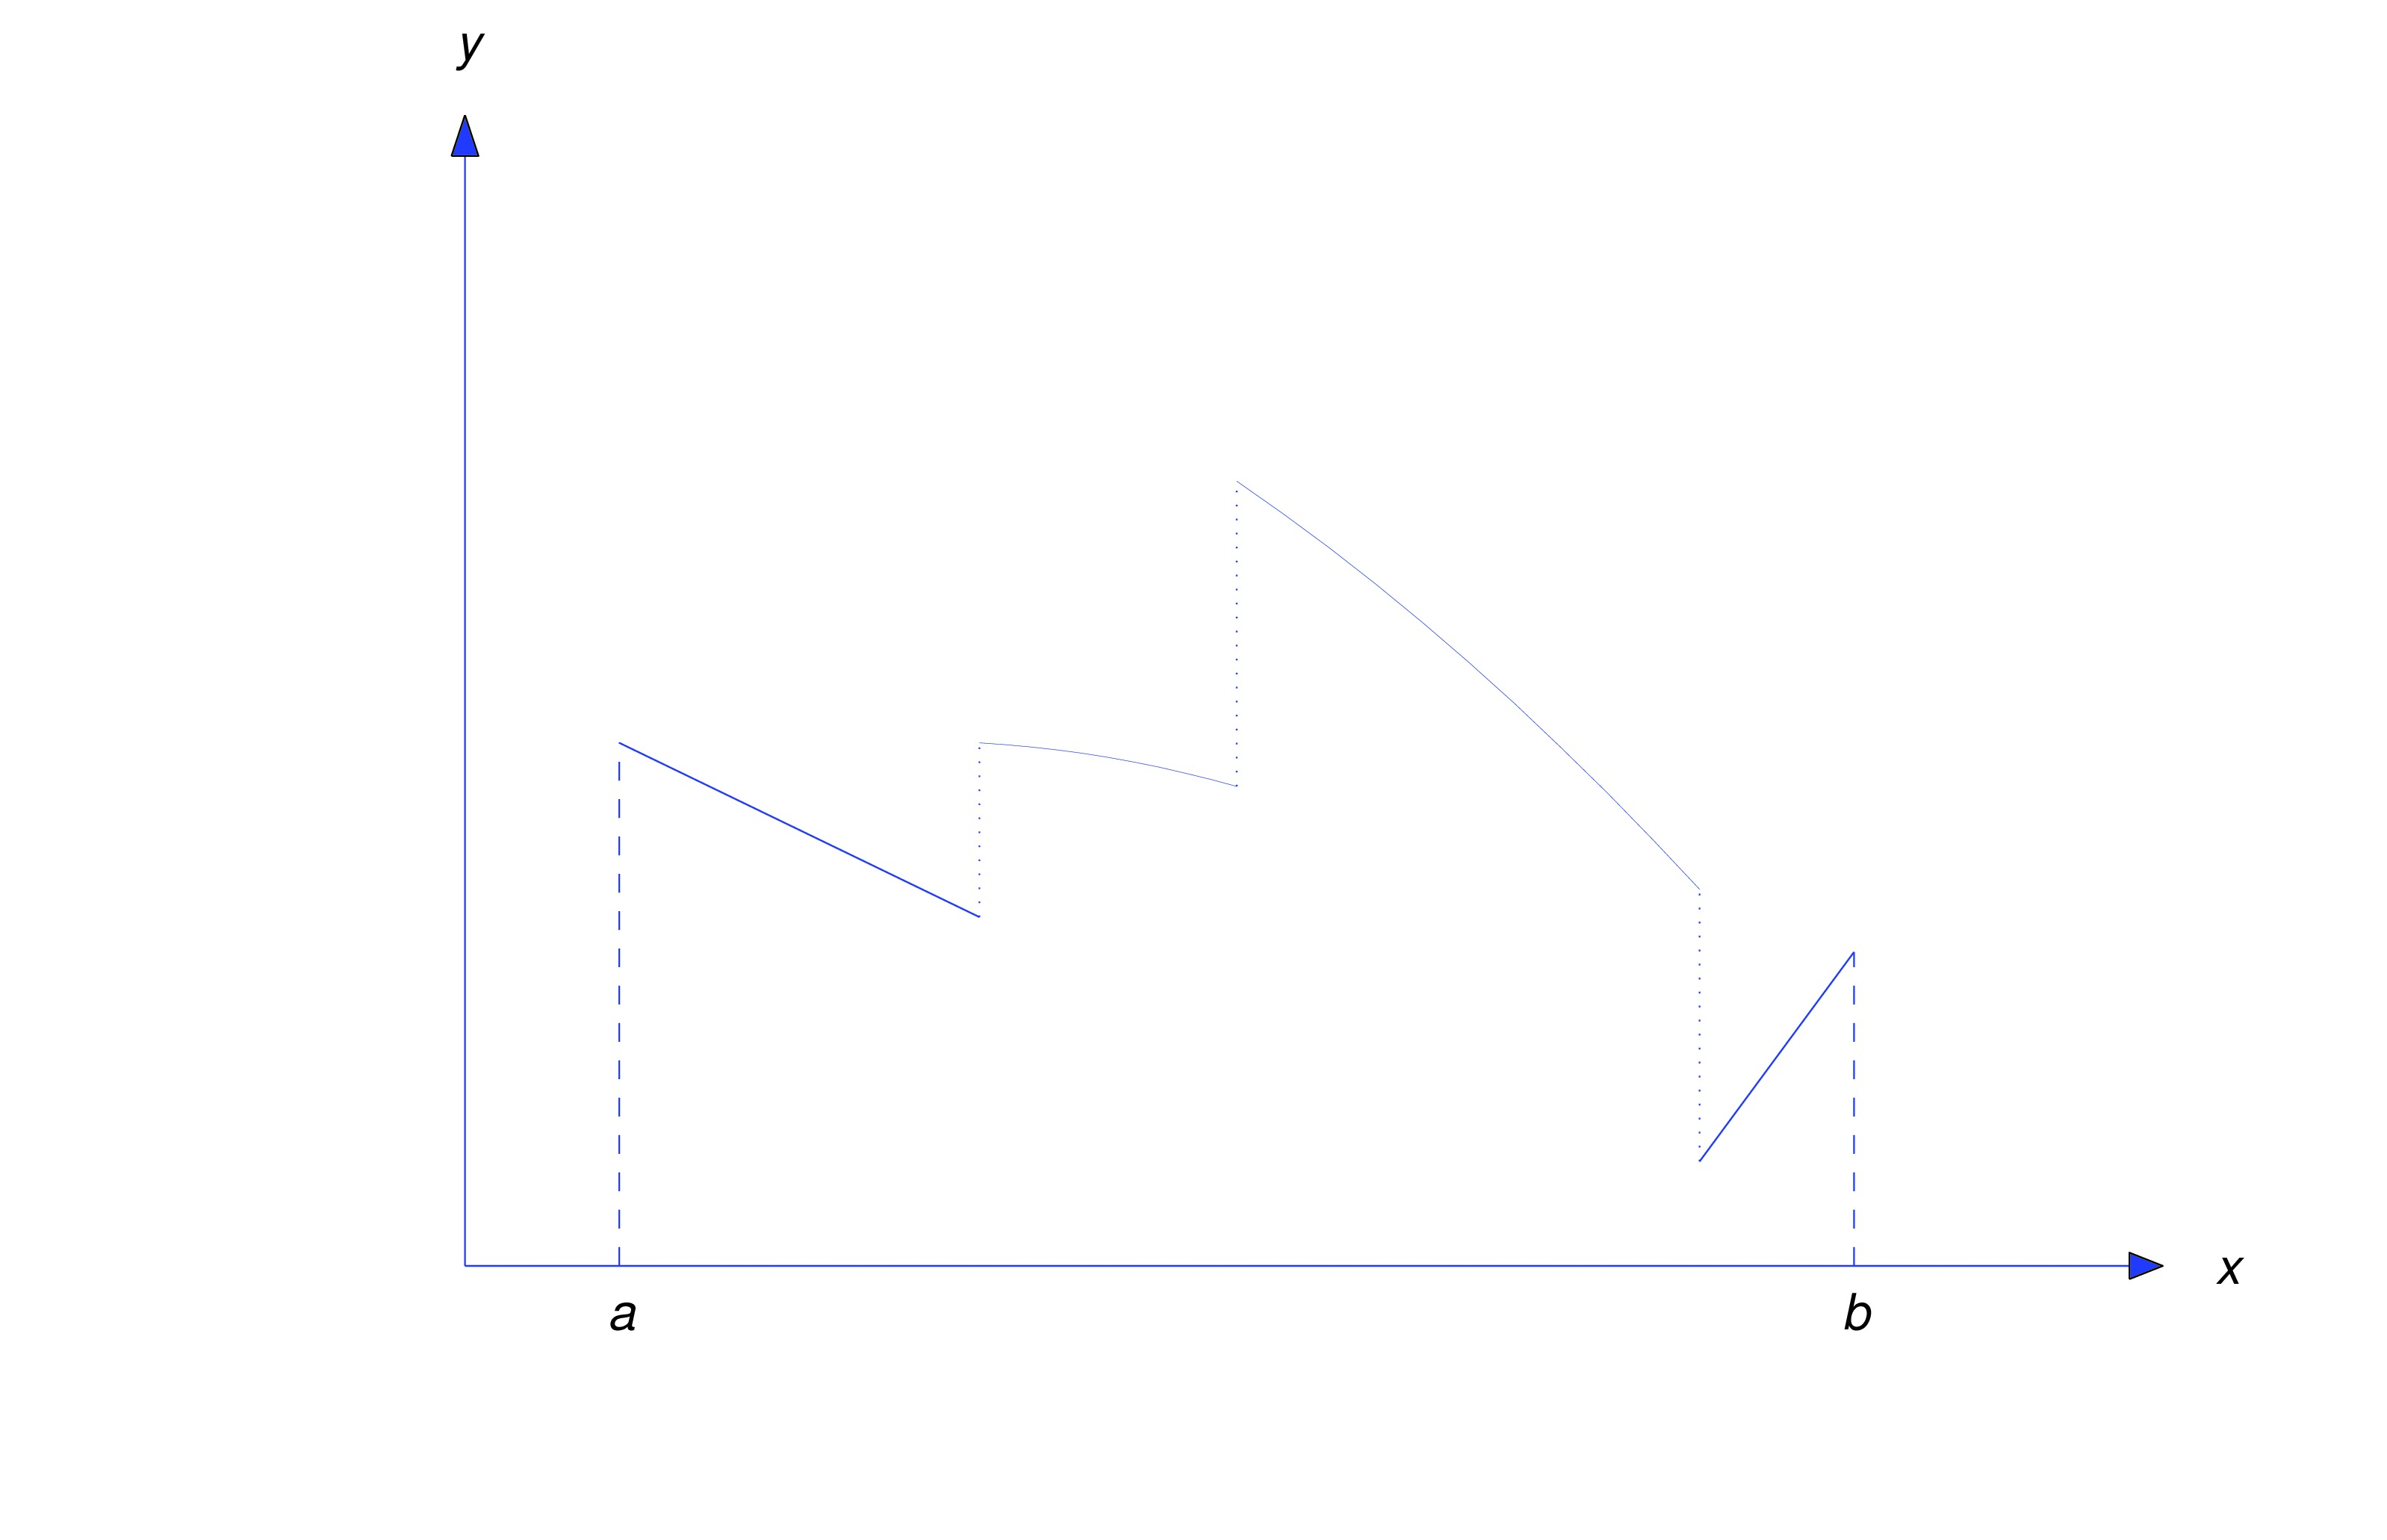
\includegraphics[bb=-78 148 689 643,width=5.67in,height=3.66in,keepaspectratio]{fig080103}}
% \caption{A piecewise continuous function on $[a,b]$}
%   \label{figure:8.1.3}
% \end{minipage}
% \end{figure}

%\color{blue}
\begin{remark}
We know from calculus that a definite integral isn't
affected by changing the values of its integrand at isolated points.
Therefore, redefining a function $f$ to make it continuous at
removable discontinuities does not change ${\cal L}(f)$.
\end{remark}
% \remark{We know from calculus that a definite integral isn't
% affected by changing the values of its integrand at isolated points.
% Therefore, redefining a function $f$ to make it continuous at
% removable discontinuities does not change ${\cal L}(f)$.}
%\color{black}

\begin{definition}\label{thmtype:8.1.4}

\begin{enumerate}
    \item\label{item:8.1.4a} % (a)
A function $f$ is said to be \textit{piecewise continuous} on a finite
closed interval $[0,T]$ if $f(0+)$ and $f(T-)$ are finite and $f$ is
continuous on the open interval $(0,T)$ except possibly at finitely
many points, where $f$ may have jump discontinuities or removable
discontinuities.
\item\label{item:8.1.4b} % (b)
A function $f$ is said to be \textit{piecewise continuous} on the
infinite interval $[0,\infty)$ if it's piecewise continuous on
$[0,T]$ for every $T>0$.
\end{enumerate}
\end{definition}

%Figure~\ref{figure:8.1.3} 
The figure below shows the graph of a typical piecewise
continuous function.

\begin{image}
 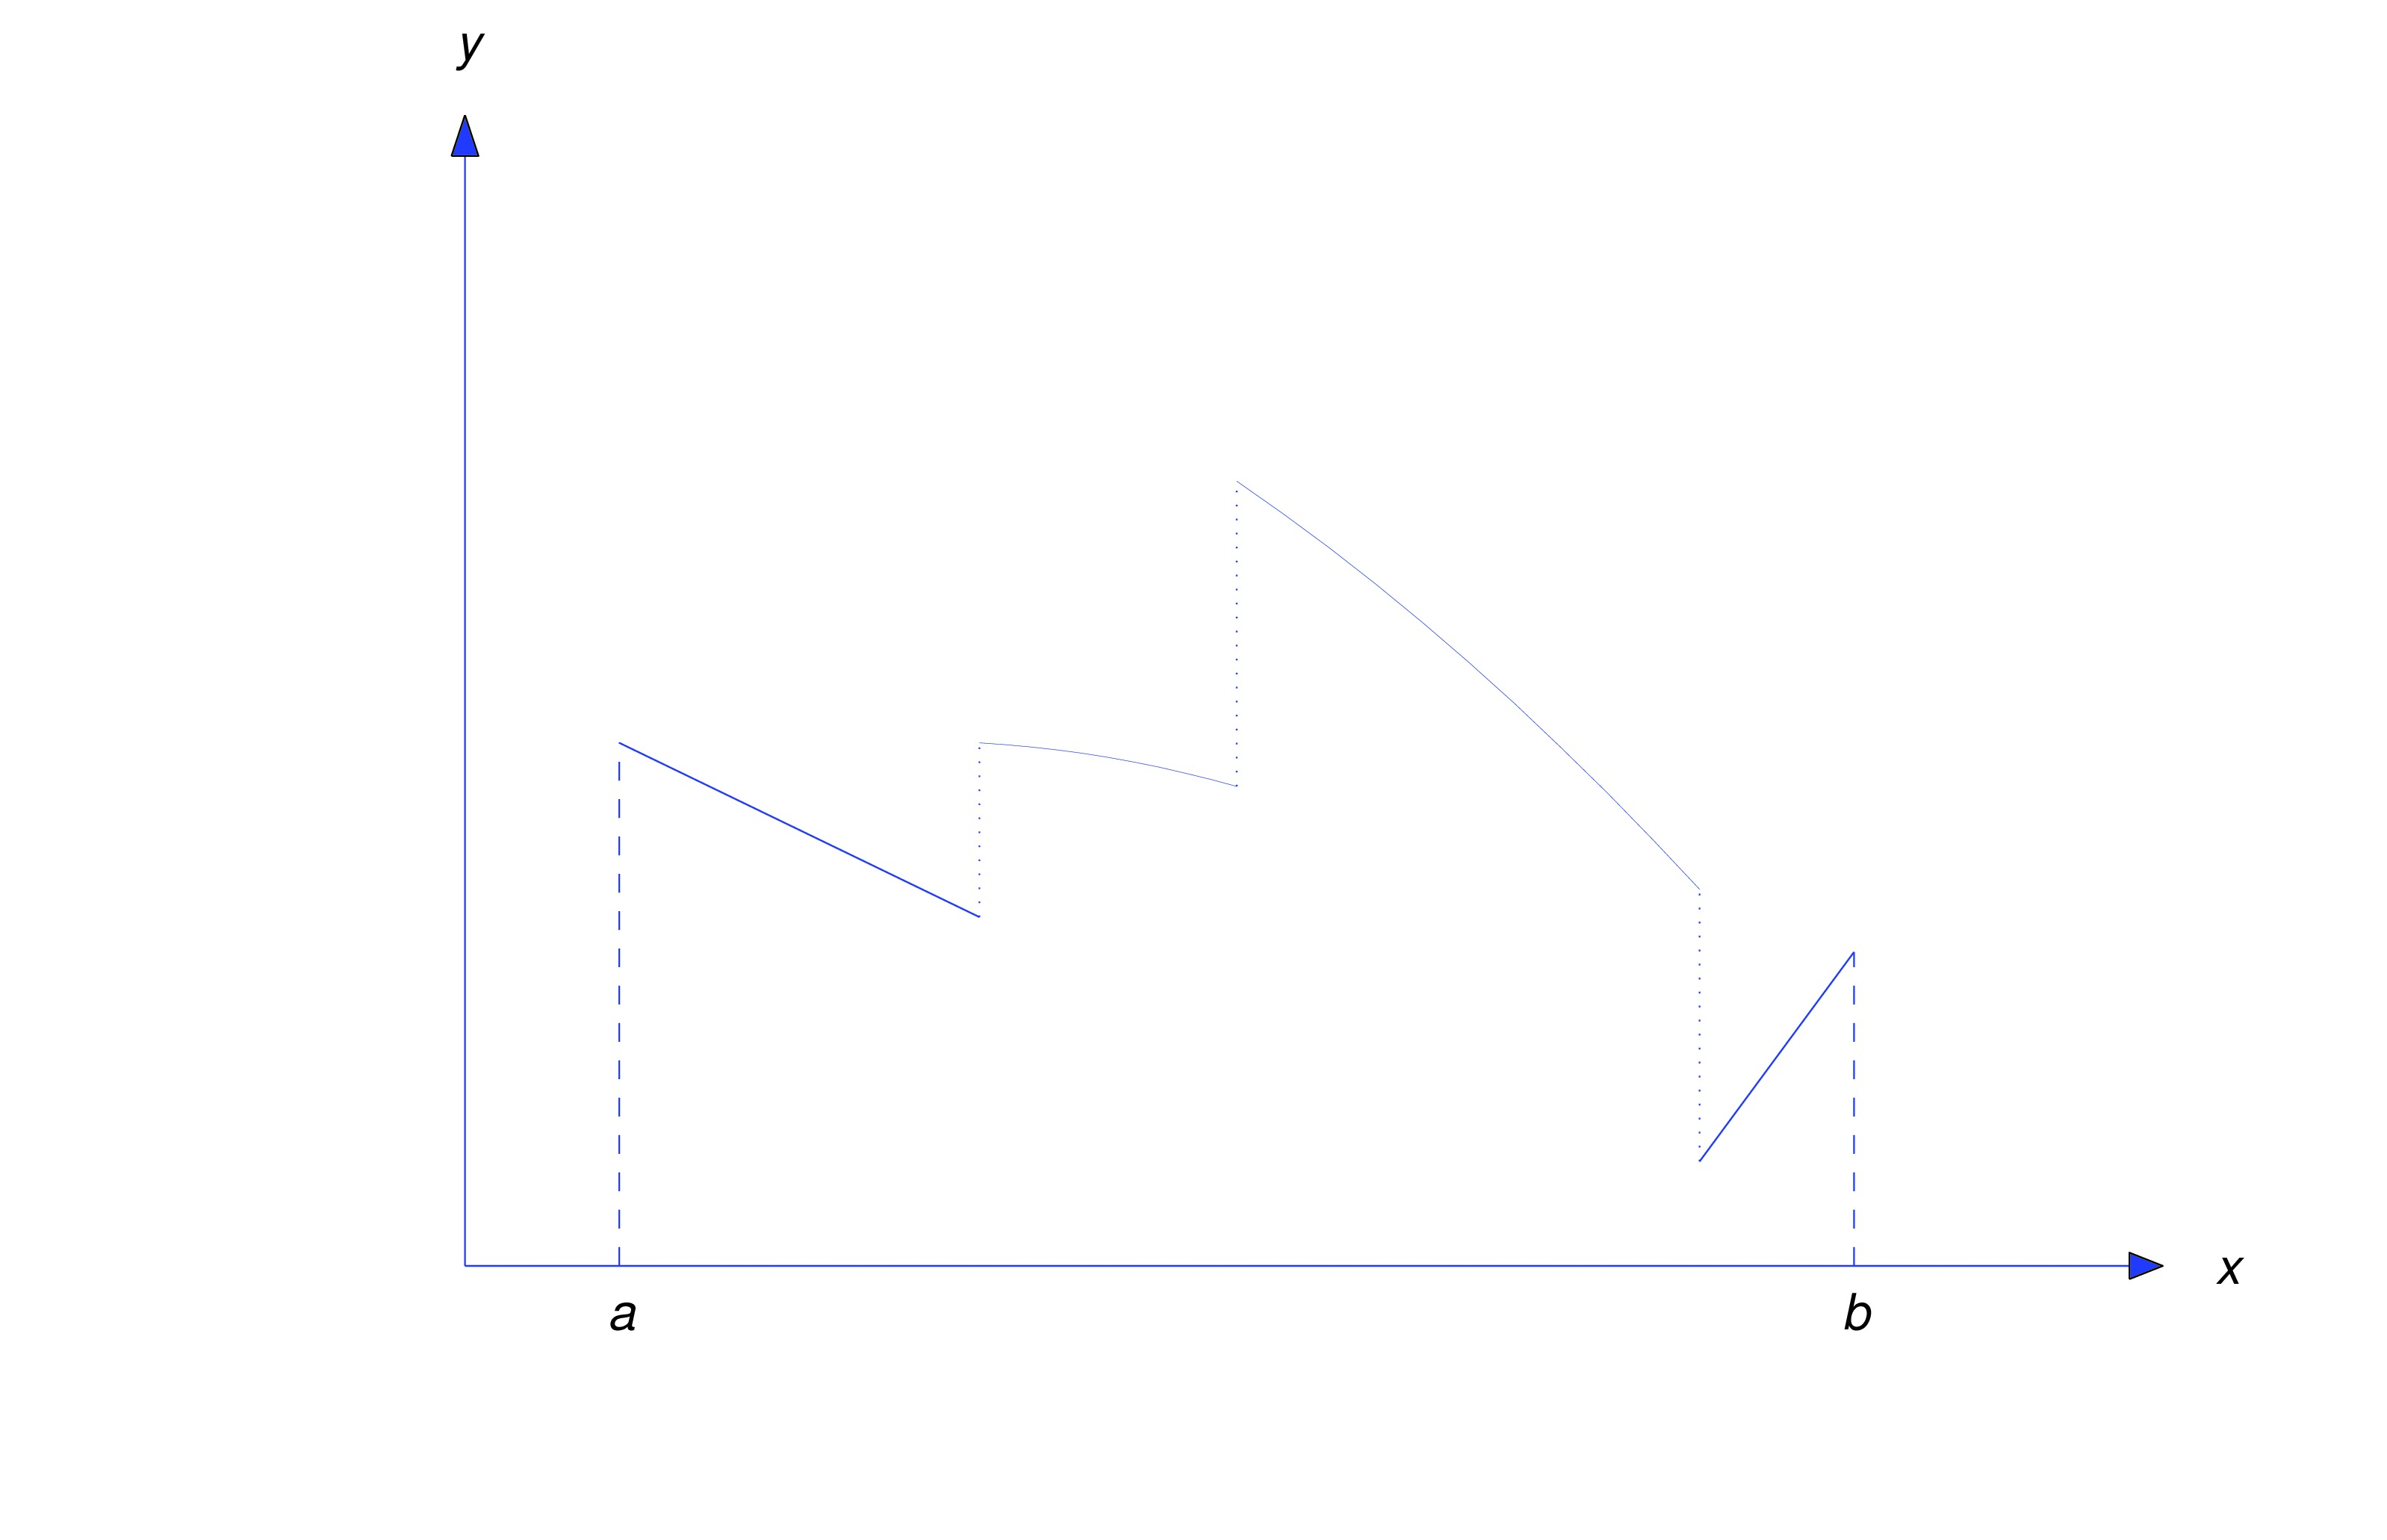
\includegraphics[height=1.5in]{fig080103.jpg}
 \end{image}


It is shown in calculus that if a function is piecewise continuous on
a finite closed interval then it's integrable on that interval. But
if $f$ is piecewise continuous on $[0,\infty)$, then so is $e^{-st}f
(t)$, and therefore
$$
\int_0^T e^{-st}f(t)\,dt
$$
exists for every $T>0$. However, piecewise continuity alone does not
guarantee that the improper integral
\begin{equation}\label{eq:8.1.13}
\int_0^\infty e^{-st}f(t)\,dt=\lim_{T\rightarrow\infty}\int_0^T e^{-st}f(t)\,
dt
\end{equation}
converges for $s$ in some interval $(s_0,\infty)$. For example, we
noted earlier that \eqref{eq:8.1.13} diverges for all $s$ if
$f(t)=e^{t^2}$. Stated informally, this occurs because $e^{t^2}$
increases too rapidly as $t\rightarrow\infty$. The next definition
provides a constraint on the growth of a function that guarantees
convergence of its Laplace transform for $s$ in some interval
$(s_0,\infty)$ .

\begin{definition}\label{thmtype:8.1.5} A
function $f$ is said to be
\textit{of exponential order} $s_0$ if there are constants $M$ and $t_0$
such that
\begin{equation}\label{eq:8.1.14}
|f(t)|\leq Me^{s_0t},\quad t\geq t_0.
\end{equation}
In situations where the specific value of $s_0$
is irrelevant we say simply that $f$ is \textit{of exponential order}.
\end{definition}

The next theorem gives useful sufficient conditions for a function $f$
to have a Laplace transform.  
%The proof is sketched in Exercise~\ref{exer:8.1.10}.

\begin{theorem}\label{thmtype:8.1.6} If $f$
is piecewise continuous on $[0,\infty)$ and of exponential order $s_0,$
 then ${\cal L}(f)$ is defined for $s>s_0$.
\end{theorem}

%\color{blue}
\begin{remark}
We emphasize that the conditions of Theorem~\ref{thmtype:8.1.6}
 are sufficient, but \textit{not necessary}, for $f$ to have a Laplace transform. 
%  For example, Exercise~\ref{exer:8.1.14}\part{c} shows that  $f$
% may have a Laplace transform even though $f$ isn't  of exponential
% order.
\end{remark}

\begin{example}\label{example:8.1.8}
If $f$ is bounded on some interval $[t_0,\infty)$, say
$$
|f(t)| \leq M,\quad t \geq t_0,
$$
then \eqref{eq:8.1.14} holds with $s_0=0$, so $f$ is of exponential order
zero. Thus, for example, $\sin\omega t$ and $\cos \omega t$ are of
exponential order zero, and Theorem~\ref{thmtype:8.1.6} implies that
${\cal L}(\sin\omega t)$ and ${\cal L}(\cos \omega t)$ exist for
$s>0$. This is consistent with the conclusion of
Example~\ref{example:8.1.4}.
\end{example}

\begin{example}\label{example:8.1.9}
It can be shown that if $\lim_{t\rightarrow\infty}e^{-s_0t}f(t)$ exists and is
finite then $f$ is of exponential order $s_0$.
%(Exercise~\ref{exer:8.1.9}). 
If $\alpha$ is any real number and $s_0>0$
then $f(t)=t^\alpha$ is of exponential order $s_0$, since
$$
\lim_{t\rightarrow\infty}e^{-s_0t}t^\alpha=0,
$$
by L'H\^opital's rule. If $\alpha\geq 0$, $f$ is also
continuous on $[0,\infty)$. Therefore Exercise~\ref{exer:8.1.9} and
Theorem~\ref{thmtype:8.1.6} imply that ${\cal L}(t^\alpha)$ exists for
$s\geq s_0$. However, since $s_0$ is an arbitrary positive number, this
really implies that ${\cal L}(t^\alpha)$ exists for all $s>0$. This is
consistent with the result of Example~\ref{example:8.1.2}.
% and
% Exercises~\ref{exer:8.1.6} and \ref{exer:8.1.8}.
\end{example}

\begin{example}\label{example:8.1.10}
Find the Laplace transform of the piecewise continuous function
$$
f(t)=\left\{\begin{array}{cl} 1,&0\leq t<1,\\  -3e^{-t},&t\geq
1.\end{array}\right.
$$
\begin{explanation}
Since $f$ is defined by different formulas
on $[0,1)$ and $[1,\infty)$, we write
$$
 F(s)=\int_0^\infty e^{-st} f(t)\,dt
=\int_0^1e^{-st}(1)\,dt+\int_1^\infty
e^{-st}(-3e^{-t})\,dt.
$$
Since
$$
\int_0^1e^{-st}\,dt=\left\{\begin{array}{cl}\frac{{1-e^{-s}}{s}},&\quad s\neq 0,\\ 1,&\quad s=0,\end{array}\right.
$$
 and
$$
\int_1^\infty e^{-st}(-3e^{-t})\,dt=-3\int_1^\infty
e^{-(s+1)t}\,dt=-\frac{3e^{-(s+1)}}{s+1},\quad s>-1,
$$
it follows that
$$
F(s)=\left\{\begin{array}{rl}\frac{{1-e^{-s}}{s}-3\frac{e^{-(s+1)}}{s+1}},&s>-1,\,s\neq 0,\\\hfill{1-\frac{3}{e}}\hfill,&
s=0.\end{array}\right.
$$
This is consistent with Theorem~\ref{thmtype:8.1.6}, since
$$
|f(t)|\leq 3e^{-t},\quad  t\geq 1,
$$
and therefore $f$ is of exponential order $s_0=-1$.
\end{explanation}
\end{example}

\begin{remark}
In \href{https://ximera.osu.edu/ode/main/unitStepFunction/unitStepFunction}{Trench 8.4} 
we'll develop a more efficient
method for finding Laplace transforms of piecewise continuous functions.
\end{remark}

\begin{example}\label{example:8.1.11}
We stated  earlier that
$$
\int_0^\infty e^{-st} e^{t^2} dt=\infty
$$
for all $s$, so Theorem~\ref{thmtype:8.1.6} implies that $f(t)=e^{t^2}$
is not  of exponential order, since
$$
\lim_{t\rightarrow\infty} \frac{e^{t^2}}{Me^{s_0t}}=\lim_{t\rightarrow\infty} \frac{1}{M} e^{t^2-s_0t}=\infty,
$$
so
$$
e^{t^2}>Me^{s_0t}
$$
for sufficiently large values of $t$, for any choice of $M$ and $s_{0}$
%(Exercise~\ref{exer:8.1.3}).
\end{example}


\section*{Text Source}
Trench, William F., "Elementary Differential Equations" (2013). Faculty Authored and Edited Books \& CDs. 8. (CC-BY-NC-SA)

\href{https://digitalcommons.trinity.edu/mono/8/}{https://digitalcommons.trinity.edu/mono/8/}


\end{document}